% =====================================================================
%  RoPART — MSc Computing Interim Report (SCAFFOLD)
%  Maciej Kuczek, Imperial College London, Department of Computing (70081)
%
%  This file is a STRUCTURE-ONLY scaffold. Every section contains a
%  \guide{...} note describing what to write and which references to draw
%  on — it renders as a grey italic "[Writing guide]" block so it is easy
%  to spot and delete. Replace each guide with your own prose, then remove
%  the macro. The body is intentionally NOT written.
%
%  Build:  pdflatex interim_report  ->  bibtex interim_report
%          ->  pdflatex x2
%  Referencing: Vancouver (numbered, in order of appearance). We use
%  unsrtnat as a portable approximation; swap in a vancouver.bst if your
%  TeX distribution ships one (see the \bibliographystyle line below).
% =====================================================================
\documentclass[11pt,a4paper]{report}

\usepackage[T1]{fontenc}
\usepackage[utf8]{inputenc}
\usepackage[british]{babel}
\usepackage[margin=2.5cm]{geometry}
\usepackage{amsmath,amssymb}
\usepackage{graphicx}
\graphicspath{{figures/}}
\usepackage[section]{placeins} % confine floats to the section they appear in
\usepackage{booktabs}
\usepackage{enumitem}
\usepackage{xcolor}
\usepackage[numbers,sort&compress]{natbib}
\usepackage[colorlinks=true,linkcolor=black,citecolor=black,urlcolor=blue]{hyperref}
\usepackage{xurl}

% --- Writing-guide macro: delete the macro use as you fill each section ---
\newcommand{\guide}[1]{%
  \par\smallskip
  \noindent{\color{gray!85!black}\small\itshape\textbf{[Writing guide]}~#1}%
  \par\smallskip
}

\begin{document}

% =====================================================================
%  TITLE PAGE
% =====================================================================
\begin{titlepage}
  \centering
  \vspace*{1.5cm}

  {\large Imperial College London \\[0.3em] Department of Computing\par}
  \vspace{2.0cm}

  {\LARGE\bfseries RoPART: Relative Orientation in \\[0.4em]
   Off-Grid Self-Supervised Learning\par}
  \vspace{1.0cm}

  {\large\itshape Extending PART from Translation to Rigid Motion\par}
  \vspace{0.4em}
  {\normalsize\itshape (RoPART --- Rotation + PART)\par}
  \vspace{2.0cm}

  {\large Maciej Kuczek\par}
  \vspace{0.4cm}
  {\normalsize MSc Computing --- Individual Project (70081)\par}
  \vspace{2.0cm}

  \begin{tabular}{rl}
    Supervisor:    & \textit{[supervisor name]} \\[0.3em]
    Second marker: & \textit{[second-marker name]} \\
  \end{tabular}

  \vfill
  {\normalsize Interim Report\par}
  {\normalsize \today\par}
\end{titlepage}

% =====================================================================
%  TABLE OF CONTENTS
% =====================================================================
\tableofcontents
\clearpage

% =====================================================================
%  CHAPTER 1 — INTRODUCTION
% =====================================================================
\chapter{Introduction}
The deep learning revolution of the last decade was made possible by a combination of three factors. First, advances in graphics processing units (GPUs) and parallel computing allowed for faster processing of large amounts of data. Second, architectural advances such as convolutional neural networks (CNNs), new regularisation techniques, and better activation functions improved the trainability and reliability of models. Third, large amounts of labelled training data allowed the models to actually learn rather than memorise. 

In 2026, compute is still growing thanks to companies such as Nvidia and AMD. Frontier labs such as OpenAI or DeepMind are hard at work researching new architectures and techniques. Labelled data, however, remains elusive and expensive, often requiring alternative approaches. One such approach is self-supervised learning (SSL), which relies on leveraging unlabelled data and pretext tasks which, when solved, provide a supervisory signal to the network.

There are many different types of pretext tasks - some remove parts of an image, some rotate the image, some remove colour - but the goal is the same: to force the network to learn complex representations of images without a human label. In particular, spatial/position pretext tasks are important as the image composition and the relationship of objects in an image can be a powerful source of information. PART (\textbf{PA}irwise \textbf{R}elative \textbf{T}ranslations)~\cite{part} is one such pretraining method that leverages relative transformations between two image patches. That method predicts relative translation only ($\Delta x,\Delta y$) with rotation left as future work - which is what this project sets out to add.

\section{Problem and context}
Most spatially-aware tasks involve a grid structure. To give some examples, Masked AutoEncoder (MAE)~\cite{mae} slices an image into a grid of patches and then masks some of them. The pretext task is to then reconstruct the missing patches. DropPos~\cite{droppos} masks some patches on a grid then drops information about absolute patch positions and tasks the network with recovering the missing positions. The pretext task in Doersch et al.'s~\cite{context2015} context prediction tasks the model with predicting the relative position of patches while still being confined to a grid.

The novel contribution of PART~\cite{part} is to sample the patches untethered to a grid and to then predict the translation between two off-grid patches. Geometrically, predicting only $(\Delta x, \Delta y)$ means PART's target space is the translation subgroup of the plane. The natural unfinished step is to predict the full group of planar rigid motions, $\mathrm{SE}(2)$, by adding a relative orientation target $\Delta\varphi$ to each patch pair. The authors themselves flag this as open: they observe that seeing a lip implies a nose above it, but a \emph{rotated} lip implies a \emph{rotated} nose, and leave modelling rotations to future work (their Section~7). This matters because grid-based pretext tasks cannot express continuous geometry of this kind, yet the dominant orientation of a part relative to its neighbours is often the discriminative signal - particularly for orientation-sensitive tasks such as pose estimation or oriented object detection. To the best of current knowledge, no prior work extends a relative off-grid patch-pair pretext task to relative orientation.

\section{Aims and objectives}
The research question can be summarised as follows: does adding a relative orientation target ($\Delta \varphi$) to each patch pair yield representations that perform better on orientation-sensitive downstream tasks without degrading classification? To answer it, the following objectives will be pursued:
\begin{itemize}
    \item Design a new pretext task that adds rotation on top of translation, accounting for artefacts such as missing corners or jagged pixels, and introducing an angle-aware loss function.
    \item Implement the rotation target behind a flag so that the translation-only baseline path is unchanged, keeping any downstream effect cleanly attributable to the orientation channel.
    \item Train a Vision Transformer on the pretext task and characterise the angle channel, under appropriate controls, to verify whether the model is learning and whether its predictions obey the geometry that the true relative orientation must obey.
    \item Evaluate downstream against the translation-only baseline on a classification no-degradation check and an orientation-sensitive task.
\end{itemize}

% =====================================================================
%  CHAPTER 2 — BACKGROUND AND LITERATURE REVIEW
% =====================================================================
\chapter{Background and Literature Review}


\section{Self-supervised representation learning}
Self-supervised learning (SSL) is a learning paradigm where the supervisory tasks is generated from data itself, without needing a human-assigned label~\cite{sslsurvey}. SSL approaches can be grouped into either generative or discriminative. The goal of generative approaches is to learn distributions over a collection of data in pixel space, whereas discriminative approaches' goal is to learn representations of data with high discriminative power (similarly to supervised approaches, just without human labels). PART and the extension proposed in this project are examples of discriminative approaches.

\section{Spatial and position-based pretext tasks}
The idea that the context could be a powerful self-supervisory signal comes from text processing. Having a model learn to predict the words surrounding any given word could lead to powerful, transferable insights. Doersch et al~\cite{context2015} extended this idea to images by asking a Convolutional Neural Network (CNN) to predict the relative position of a reference patch given a target patch (Figure~\ref{fig:doersch}). This works because, for example, to predict that a patch containing a cat's left ear is to the top left of a patch containing a cat's nose the model has to build a correct representation of an object and its constituent parts. This idea was extended further by~\cite{jigsaw} where the pretext task was to solve a "jigsaw" puzzle where the model had to reassemble a picture that was sliced into patches along a grid and then shuffled (Figure~\ref{fig:jigsaw}). Once again, by the learned representations used to solve this pretext task captured semantically relevant content.

\begin{figure}[t]
  \centering
  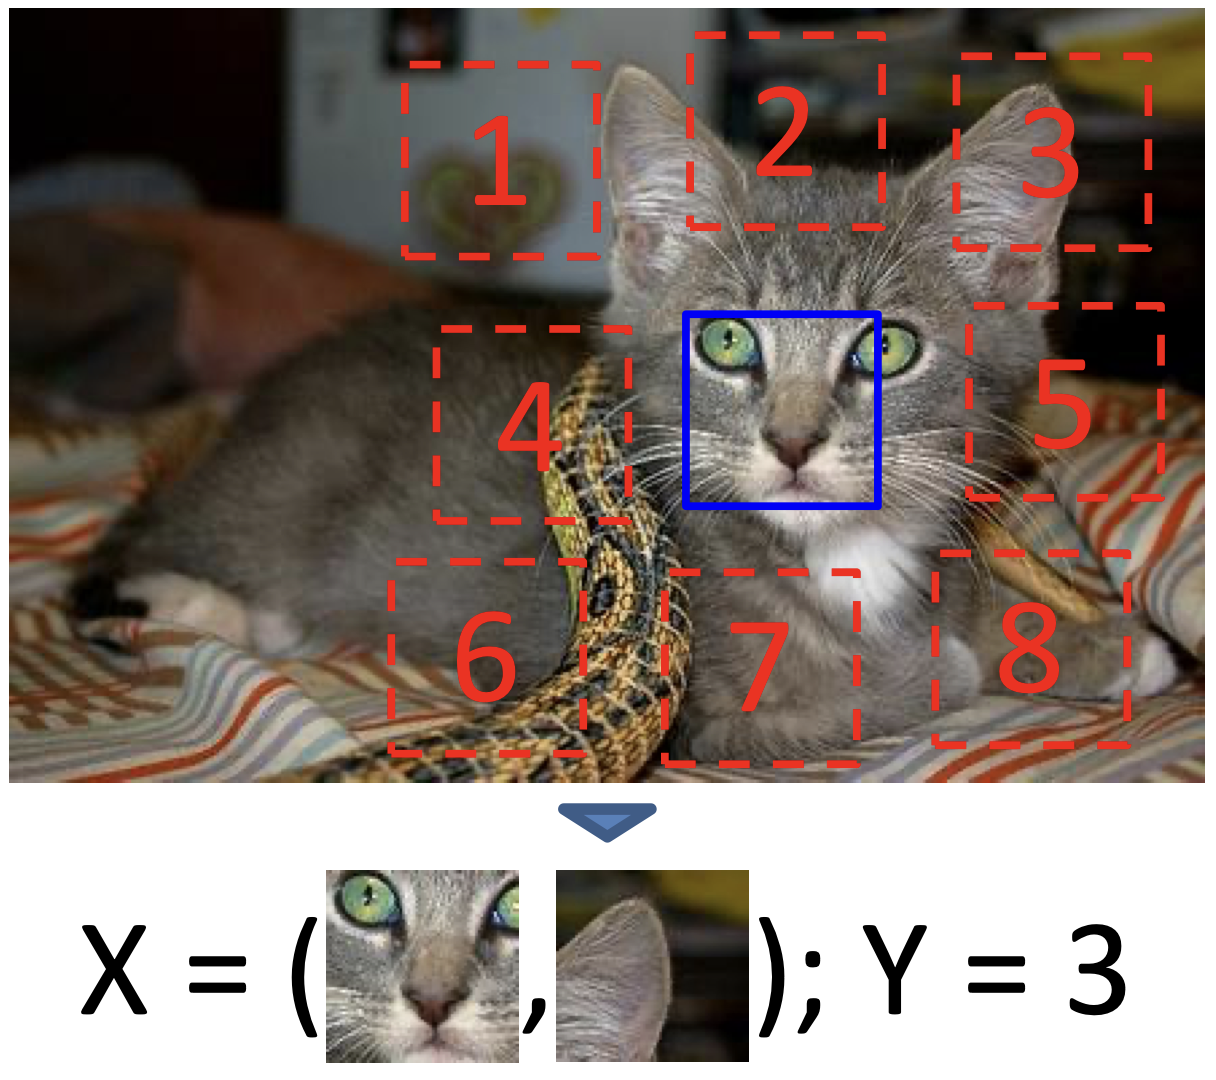
\includegraphics[width=0.45\textwidth]{Doersch.png}
  \caption[Relative context prediction]{Relative context prediction of Doersch et
  al.~\cite{context2015}: given a reference patch (centre) and a neighbouring patch,
  the network predicts which of the eight surrounding grid positions the
  neighbour occupies. The positions remain confined to a fixed grid relative to the
  reference. Figure reproduced from~\cite{context2015}.}
  \label{fig:doersch}
\end{figure}

\begin{figure}[t]
  \centering
  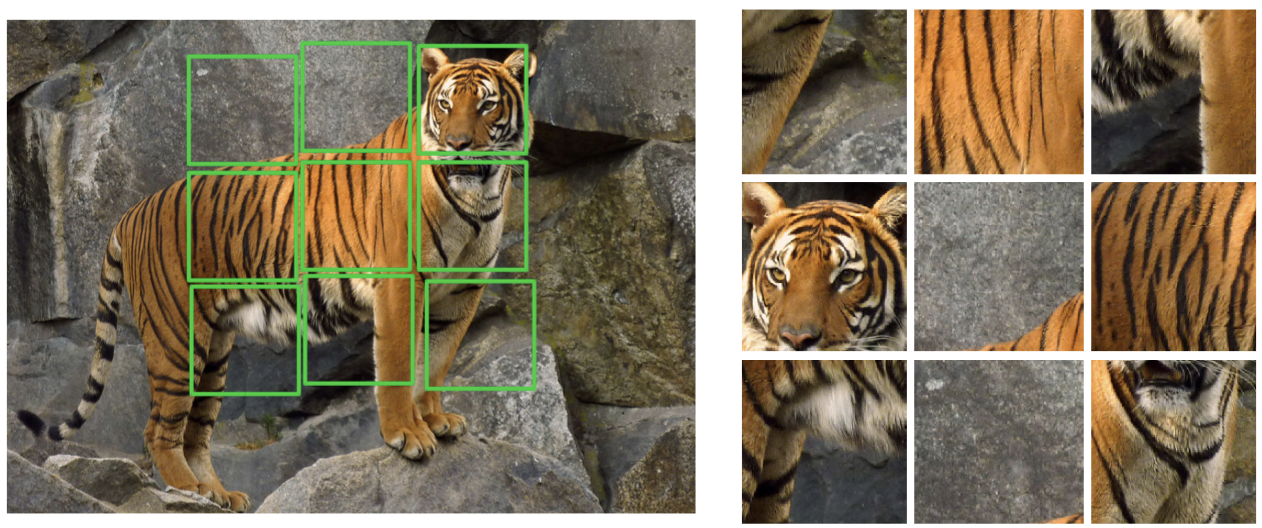
\includegraphics[width=0.6\textwidth]{Jigsaw.png}
  \caption[Jigsaw puzzle pretext task]{The jigsaw pretext task of Noroozi \&
  Favaro~\cite{jigsaw}: an image is sliced into grid tiles which are shuffled
  according to a permutation, and the network must recover the permutation that
  reassembles the original image. As with context prediction, the tiles are tied to a
  fixed grid. Figure reproduced from~\cite{jigsaw}.}
  \label{fig:jigsaw}
\end{figure}

In the transformer era, computer vision also took inspiration from NLP, this time leveraging masking. Masked AutoEncoder~\cite{mae} constructs a pretext task by masking out a subset of patches at random and then asks a vision transformer to reconstruct the missing patches - this is a generative approach operating at pixel level (Figure~\ref{fig:mae}). Notably, the patches are still confined to a fixed grid. MP3~\cite{mp3} is an example of vision transformer solving a position prediction pretext task - its goal is to predict the absolute position of a patch on a grid (Figure~\ref{fig:mp3}). The authors achieve that by removing positions, selecting random context tokens and then tasking the model with predicting absolute positions for each token. While MP3 drops all position embeddings, DropPos~\cite{droppos} drops a subset of positional embeddings, keeping the remaining ones as "anchors" (Figure~\ref{fig:droppos}).

\begin{figure}[t]
  \centering
  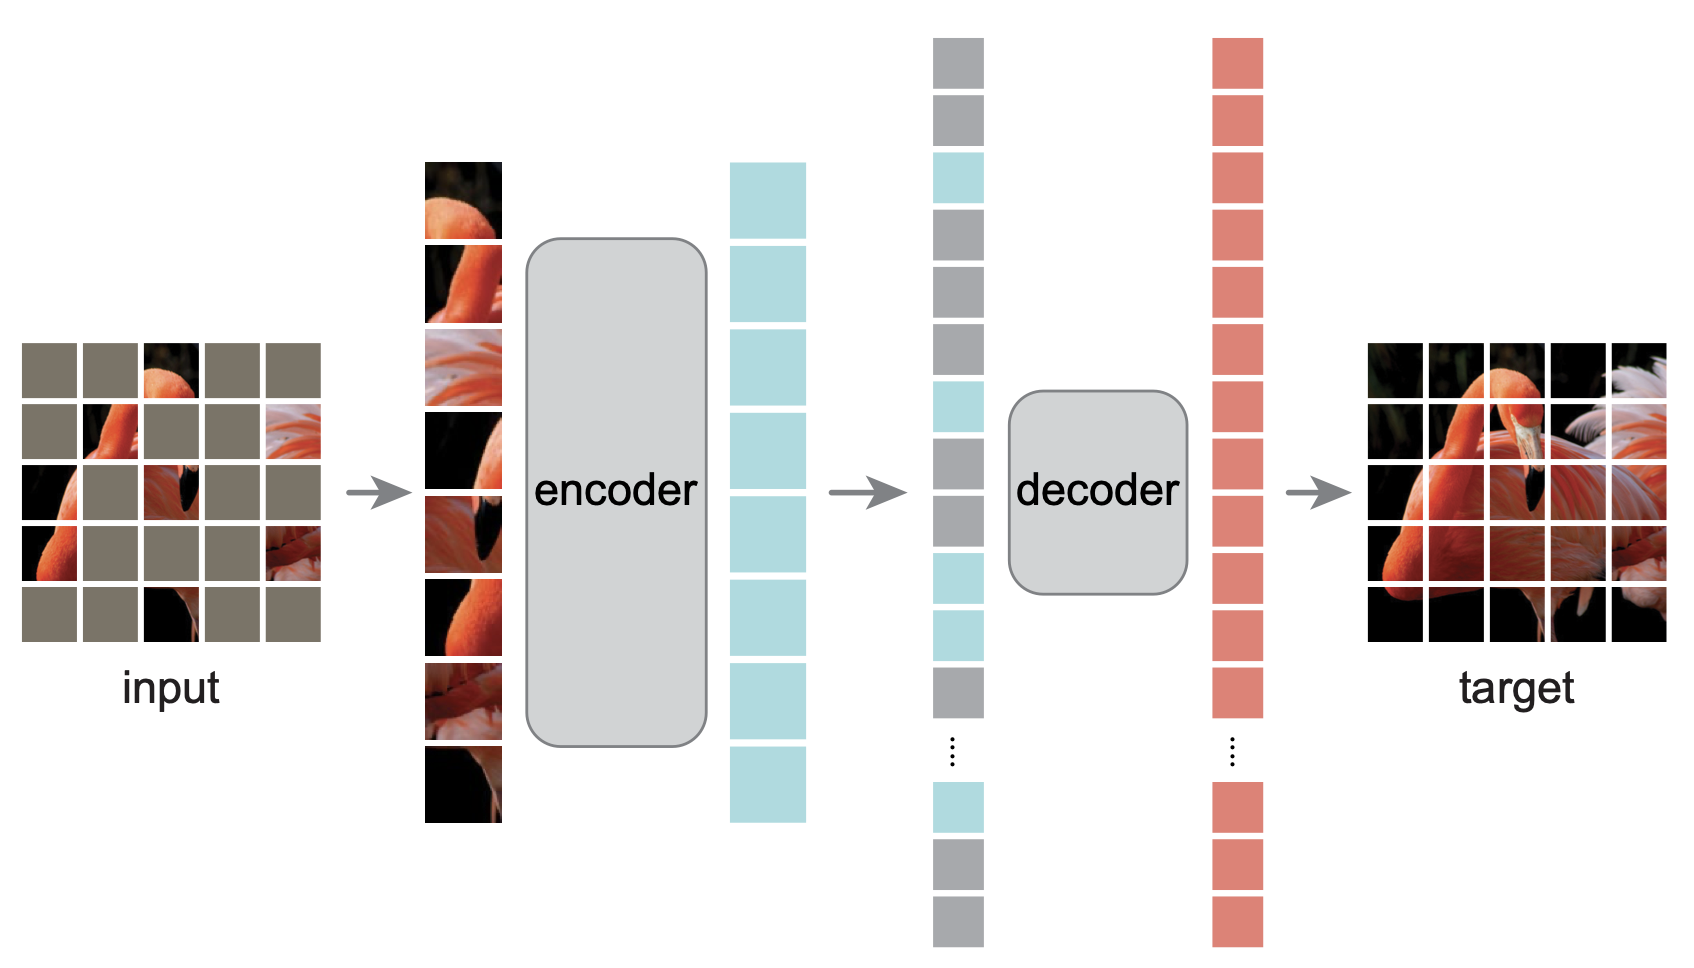
\includegraphics[width=0.6\textwidth]{MAE.png}
  \caption[Masked Autoencoder]{The Masked Autoencoder (MAE)~\cite{mae}: a large
  fraction of grid patches is masked, an encoder processes the visible patches, and
  a lightweight decoder reconstructs the missing pixels. The objective is generative
  (pixel reconstruction) and operates on a fixed grid. Figure reproduced
  from~\cite{mae}.}
  \label{fig:mae}
\end{figure}

\begin{figure}[t]
  \centering
  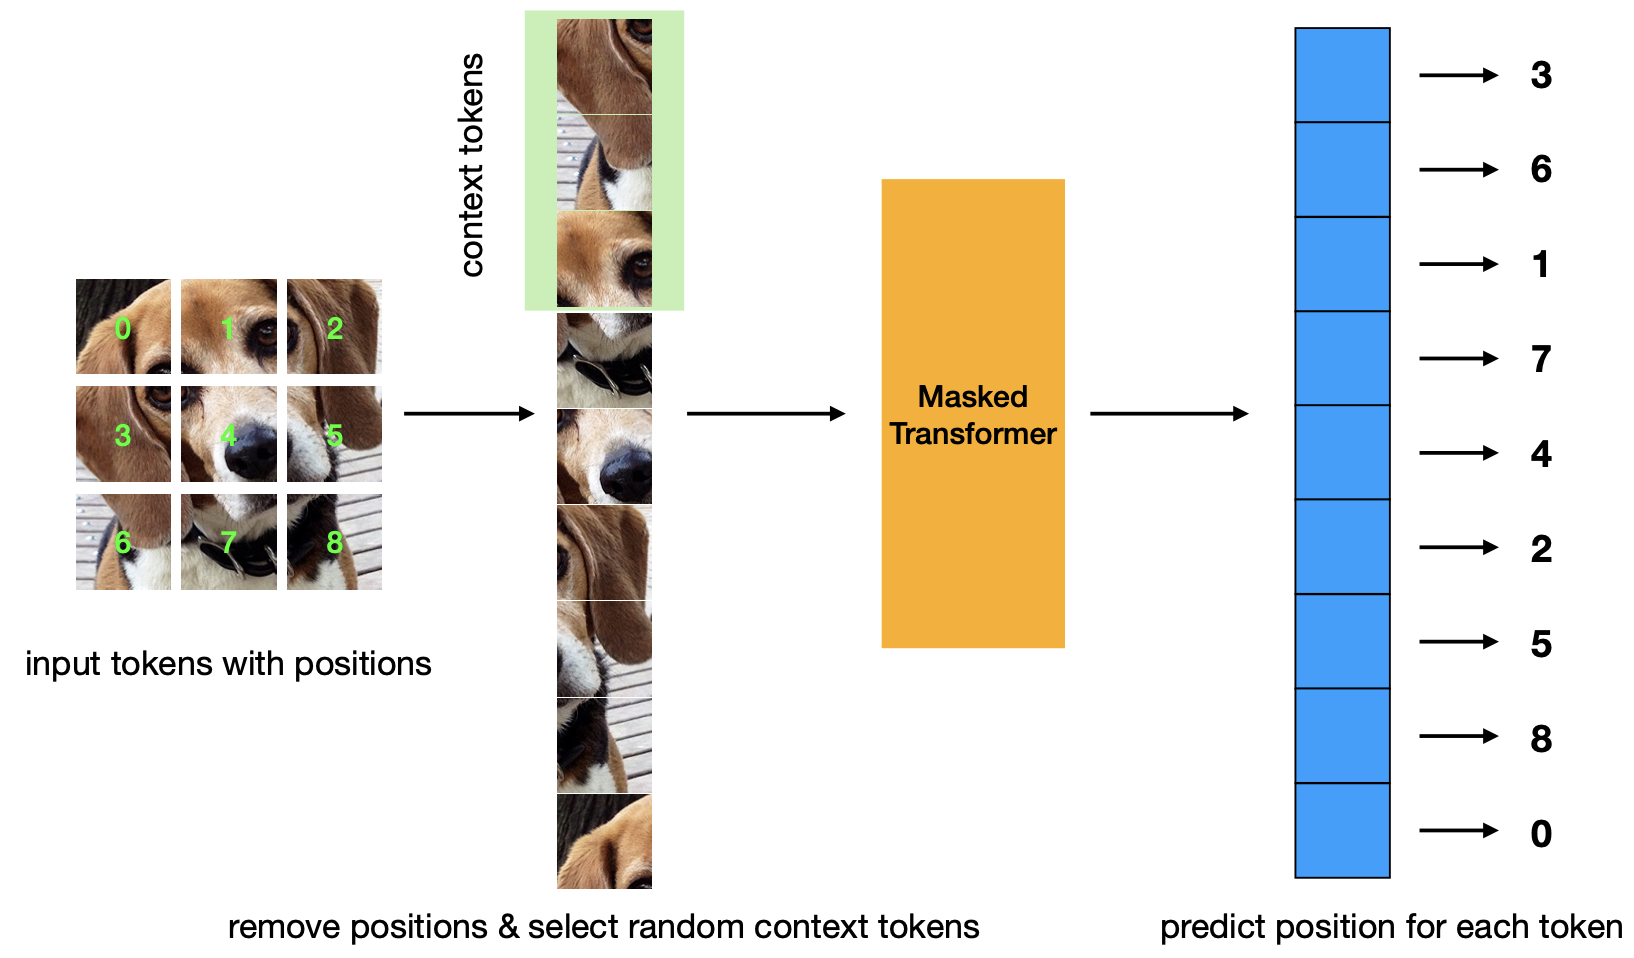
\includegraphics[width=0.6\textwidth]{MP3.png}
  \caption[MP3 position prediction]{MP3~\cite{mp3}: all positional embeddings are
  removed and the network must predict the \emph{absolute} grid position of each
  token from content alone. Figure reproduced from~\cite{mp3}.}
  \label{fig:mp3}
\end{figure}

\begin{figure}[t]
  \centering
  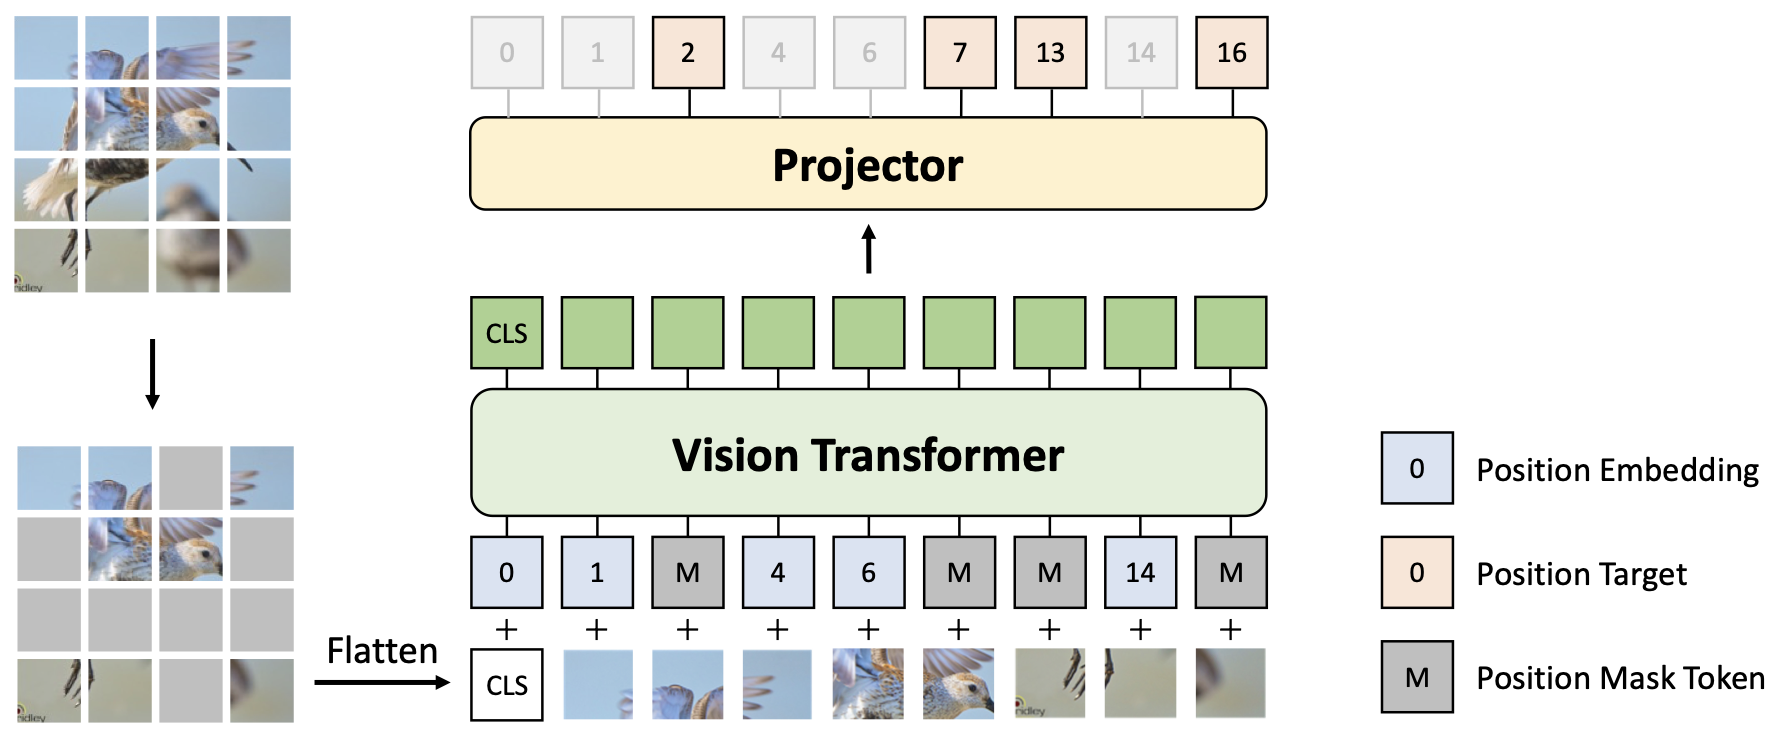
\includegraphics[width=0.72\textwidth]{DropPos.png}
  \caption[DropPos]{DropPos~\cite{droppos}: only a subset of positional embeddings is
  dropped, with the retained embeddings acting as anchors against which the dropped
  positions are recovered. The task remains one of predicting absolute positions on a
  fixed grid. Figure reproduced from~\cite{droppos}.}
  \label{fig:droppos}
\end{figure}

Crucially, all methods mentioned above are confined to a fixed grid and predict positions or reconstruct masked content on that fixed grid.

\section{PART: relative composition of off-grid patches}
\textbf{PA}irwise \textbf{R}elative \textbf{T}ranslations~\cite{part} is a pretraining method that is not based on a grid (Figure~\ref{fig:part}). Given that this paper is the base of this project, a more detailed treatment is required.

\begin{figure}[t]
  \centering
  
\includegraphics[width=\textwidth]{PART.jpg}
  \caption[The PART pipeline]{The PART pipeline~\cite{part}: patches are sampled at
  random continuous (off-grid) positions and embedded by a ViT \emph{without}
  positional embeddings; a cross-attention relative encoder then predicts the
  relative translation $(\Delta x,\Delta y)$ between sampled patch pairs, supervised
  with an MSE loss. The geometry of the pair, rather than an absolute grid position,
  provides the supervisory signal. Figure reproduced from~\cite{part}.}
  \label{fig:part}
\end{figure}

First, given an image, $N$ random patches are extracted, where the top-left coordinates of patch $s$, $(x_s,y_s)$ are drawn uniformly across the image. The patches are of size $P$ (therefore, the bottom-right coordinates are given by $(x_s+P,y_s+P)$). Because the patches are sampled uniformly and off-grid, masking occurs naturally. Note that no positional embeddings are used.

The goal is to learn the translation between any pair of patches (considering the width $w_\text{ref}$ and height $h_\text{ref}$ of the reference patch):

$$\theta_{\text{ref},\text{tgt}}=\begin{bmatrix} \Delta x \\ \Delta y \end{bmatrix}_{\text{ref},\text{tgt}}=\begin{bmatrix} (x_\text{tgt}-x_\text{ref})/w_{\text{ref}} \\ (y_\text{tgt}-y_\text{ref})/h_\text{ref} \end{bmatrix}_{\text{ref},\text{tgt}}$$

Overall, $N=\frac{H\times W}{P^2}$ patches are sampled (this is the same number that a grid would produce) and reshaped into the original image size $\hat{I}\in \mathbb{R}^{H\times W\times C}$ where $C$ is the number of channels. The patches are then flattened and linearly projected into $X\in\mathbb{R}^{N\times d}$ (standard ViT procedure). $X$ then goes through ViT to obtain learned embeddings $X'\in \mathbb{R}^{N\times d}$.

To construct a relative encoder architecture, random subset of patch indices is sampled, $S\in\mathbb{N}^{2\times \#\text{pairs}}$, with $S_0$ as the index of reference patches and $S_1$ as the index of target patches. Afterwards, the reference and target embeddings are gathered and concatenated to obtain $\hat{X}=\text{concat}(X'_{S_0},X'_{S_1})\in\mathbb{R}^{\#\text{pairs}\times 2d}$. Finally, $\hat{X}$ goes through a linear projection to bring it to $\hat{X}\in \mathbb{R}^{\#\text{pairs}\times d}$ so each pair is now $d$-dim query vector. $X'$ is fed as both the key and value. This yields attention: $\hat{\theta}=\text{attn}=\text{softmax}(\frac{\hat{X}X'^T}{\sqrt{d}})X'$. After one final linear projection, one obtains $\hat{\theta}\in\mathbb{R}^{\#\text{pairs}\times2}$.

Finally, mean squared loss is used:
$$\mathcal{L}_{MSE}=\frac{1}{2\times\#\text{pairs}}\sum^2_{k=1}\sum^{\#\text{pairs}}_{m=1}(\theta_{mk}-\hat{\theta}_{mk})^2$$

The authors also show that the framework is extensible by adding relative scale and aspect ratio terms $\Delta w,\Delta h$. This extends the objective to:
$$\theta_{\text{ref},\text{tgt}}=\begin{bmatrix} \Delta x \\ \Delta y \\ \Delta w \\ \Delta h \end{bmatrix}_{\text{ref},\text{tgt}}=\begin{bmatrix} (x_\text{tgt}-x_\text{ref})/w_{\text{ref}} \\ (y_\text{tgt}-y_\text{ref})/h_\text{ref} \\ w_\text{tgt}/w_\text{ref} \\ h_\text{tgt}/h_\text{ref} \end{bmatrix}_{\text{ref},\text{tgt}}$$
The authors note that this delays the convergence of $\Delta x,\Delta y$ compared to the baseline. 

Crucially, the model learns symmetrical relationships, i.e. if patch $P_i$ predicts $(\Delta x,\Delta y)$ relative to $P_j$, then $P_j$ predicts $(-\Delta x,-\Delta y)$ relative to $P_i$. The method is also capable of estimating patch uncertainty by checking the agreement of different reference patches on the relative position of a target patch - with "easy" patches being consistently placed at the same location.

The authors conclude the paper with several future directions such as hierarchical multi-scale learning, extensions to other tasks, and - most importantly to this project - modelling rotations.

\section{Rotation in self-supervision and in architectures}
Rotation can be an SSL objective in itself. In RotNet~\cite{rotnet} the whole image is rotated globally by $0^{\circ},90^{\circ},180^{\circ},270^{\circ}$ and the network must classify which of the four rotations was applied (Figure~\ref{fig:rotnet}). This approach does not introduce low-level visual artefacts and exhibits well-posedness. Interestingly, adding rotations of $45^{\circ},135^{\circ},225^{\circ},315^{\circ}$ degrades CIFAR-10 classification accuracy - the authors attribute this degradation to the fact that 8 rotations are not distinguishable enough and/or the fact that visual artefacts are introduced. Later work refined the signal - Feng et al.~\cite{rotdecouple} decouple rotation-dependent from rotation-invariant features. On the other hand, Misra and van der Maaten~\cite{pirl} argue that representations should be invariant to such transformations rather than predict them. Across this line of research, rotation is a global, absolute, image-level signal predicted as a few discrete classes. The orientation studied here is instead relative between a patch pair, local, and continuous; to the best of current knowledge no prior work supervises relative orientation between off-grid patch pairs.

\begin{figure}[t]
  \centering
  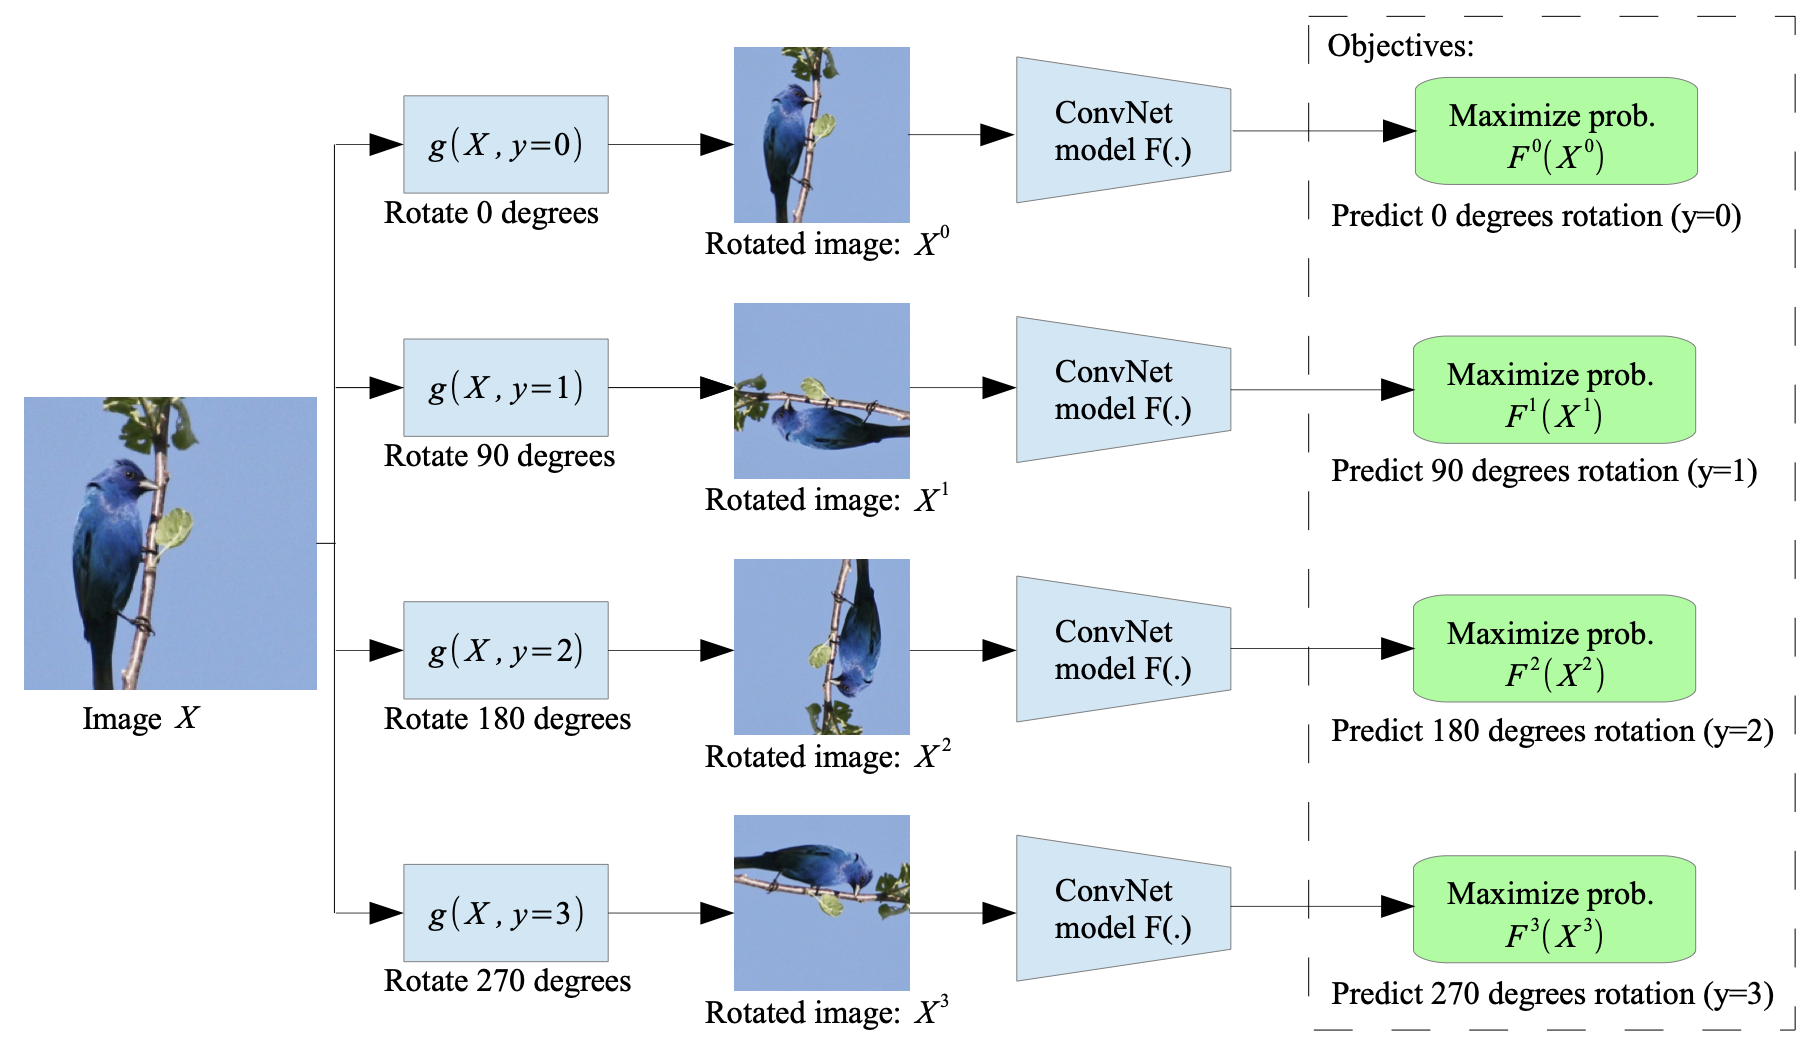
\includegraphics[width=0.6\textwidth]{RotNet.png}
  \caption[RotNet]{RotNet~\cite{rotnet}: the input image is rotated by one of four
  multiples of $90^{\circ}$ and the network is trained to recognise the applied
  rotation. The target is a single \emph{global}, \emph{discrete}, image-level
  rotation --- in contrast to the continuous, pairwise, part-relative orientation
  this project proposes. Figure reproduced from~\cite{rotnet}.}
  \label{fig:rotnet}
\end{figure}

\section{Representing and regressing rotation}
To represent rotation, a simple direct angle regression may be used. This is a poor neural target: an angle is a point on the unit circle, so any scalar parametrisation is discontinuous at the $\pm\pi$ wrap-around, where two near-identical orientations sit at opposite ends of the range. The network must then approximate a discontinuous function, which yields large gradients at the seam and penalises errors that reflect no real geometric difference; Zhou et al.~\cite{rotcont} show such discontinuous representations are harder to learn. Encoding the angle on the unit circle as $(\cos\Delta\varphi,\sin\Delta\varphi)$ removes the seam and is therefore a better target, supervised either by an MSE on the two components or by a cosine loss $1-\cos(\Delta\hat\varphi-\Delta\varphi)$. This representation also fixes how the intrinsic metrics are computed: the predicted angle is recovered from the network's $(\cos,\sin)$ outputs, the angular error is measured as the difference from the true angle wrapped around the circle into $(-\pi,\pi]$, and the negative-symmetry and compositional-consistency checks are likewise evaluated on the circle rather than on raw scalar differences.


\section{Multi-objective learning and loss balancing}
Predicting several relative quantities from a shared backbone is a multi-task regression. This means that channels with different units and convergence rate may interfere and a single fixed loss weighting may prove hard to tune and may not be optimal throughout training. Indeed, in PART~\cite{part} itself adding the relative scale and aspect ratio terms delayed the convergence of translation terms relative to the baseline. One established solution is to make the weighting adaptive. Kendall et al.~\cite{kendall} propose weighting each task by a learned homoscedastic uncertainty which automatically downweights noisier tasks.

\section{Orientation-sensitive downstream tasks}
The value of orientation-aware representations is clearest in domains without a canonical "up". Aerial imagery is the standard case: viewed from above, objects appear at arbitrary in-plane orientations and are often densely packed with large aspect ratios, so axis-aligned boxes localise them poorly. This motivates oriented object detection, where targets are rotated bounding boxes carrying an explicit angle. DOTA~\cite{dota} is a large-scale benchmark for this task in aerial imagery and HRSC2016~\cite{hrsc2016} a focused high-resolution dataset for oriented ship detection - both annotate and evaluate orientation directly. A representative state-of-the-art detector is Oriented R-CNN~\cite{orcnn}, which adds an oriented region proposal network that produces rotated proposals almost cost-free, reaching $75.87\%$ mAP on DOTA and $96.50\%$ mAP on HRSC2016 at $15.1$~FPS. Such results show orientation is routinely learned as a regression target on well-characterised benchmarks - the setting in which an orientation-aware pretrained backbone could be assessed, and what motivates the downstream evaluation here.

% =====================================================================
%  CHAPTER 3 — TECHNICAL ACHIEVEMENTS / PRELIMINARY WORK
% =====================================================================
\chapter{Preliminary Work and Feasibility}

\section{Reproducing the PART pipeline on a modern stack}
A short feasibility test was run on a local device (2021 M1 Pro MacBook Pro). Tech stack of torch, torchvision, and timm (PyTorch Image Models) had to be bumped up by several versions as the wheels used by the PART paper~\cite{part} do not exist for modern Python. Some minor bugfixes in the original codebase were applied as bumping up the Python version from $\leq 3.11$ to $3.12$ introduced stricter f-string parsing. Running on MPS backend, the loss was finite and monotonically decreasing. As mentioned in the original paper, scale channels ($\Delta w, \Delta h$) dropped steeply while translation channels ($\Delta x, \Delta y$) barely moved in the first couple of hundred of iterations. Based on these results, Apple-Silicon MPS will be used for local development and testing while for the full pretraining and downstream training the DoC GPU cluster will be used via Slurm.


% =====================================================================
%  CHAPTER 4 — PROJECT PLAN
% =====================================================================
\chapter{Project Plan}

\section{Approach and phases}
The work is organised into five phases, building the geometry one channel-group at a
time, simplest first, so that any downstream effect is cleanly attributable to the
orientation channel. A guiding principle throughout is that every rotation-related
addition is gated behind a \texttt{-{}-rotation} flag, so that with the flag off the
translation-only baseline path is byte-for-byte unchanged and remains a clean
control.

\begin{enumerate}
  \item \textbf{Phase 0 - Setup and baseline.} Set up the repository on a modern
  stack, reproduce the PART CIFAR-100 / ViT-S baseline, then strip it to the
  translation-only $(\Delta x, \Delta y)$ control by disabling the scale channels.

  \item \textbf{Phase 1 - RoPART: the rotation-aware pretext.} Add relative
  orientation as a $(\cos\Delta\varphi, \sin\Delta\varphi)$ target on top of the
  baseline (raising the relative head from 2 to 4 channels), with an angle-aware
  loss, continuous $\varphi$, and the interpolation control. 

  \item \textbf{Phase 2 - Does $\Delta\varphi$ learn?}
  Full-scale pretraining on the DoC GPU cluster, characterising the orientation
  channel with intrinsic metrics under the confound controls, alongside the
  following ablations:
  \begin{itemize}
    \item angle representation (e.g.\ $(\cos,\sin)$ MSE vs.\ cosine loss);
    \item frame convention (global vs.\ reference-local rotated frame);
    \item loss weighting ($w_\varphi$, fixed vs.\ uncertainty-weighted);
    \item whether adding scale $(\Delta w, \Delta h)$ helps --- evaluated last, and
    folded in only if it does.
  \end{itemize}

  \item \textbf{Phase 3 - Downstream evaluation.} Evaluate the pretrained backbone
  against the translation-only baseline on a classification no-degradation check, a
  synthetic orientation probe, and one real orientation-sensitive task.

  \item \textbf{Phase 4 - Synthesis and writing.} Unified comparison, a
  reproducible artefact (code, seeds, checkpoints, configs), and writing up.
\end{enumerate}

\section{Timeline}
The phases above map onto the calendar as shown in Table~\ref{tab:timeline}, working
back from the final report deadline of 9 September 2026.

\begin{table}[h]
  \centering
  \begin{tabular}{@{}lll@{}}
    \toprule
    Phase & Dates & Milestone / deliverable \\
    \midrule
    Phase 0 & 06 Jun -- 21 Jun & Baseline reproduced; translation-only control \\
    Phase 1 & 22 Jun -- 12 Jul & Rotation pretext $(\Delta x,\Delta y,\Delta\varphi)$ training at scale \\
    Phase 2 & 13 Jul -- 02 Aug & Ablations + intrinsic metrics under confound controls \\
    Phase 3 & 03 Aug -- 23 Aug & Downstream evaluation vs.\ baseline \\
    Phase 4 & 24 Aug -- 9 Sep & Synthesis; presentation; report \\
    \bottomrule
  \end{tabular}
  \caption{Project timeline. The hard deadline is the final report on 9 September 2026.}
  \label{tab:timeline}
\end{table}

\section{Evaluation and success criteria}
Success is judged against the translation-only $(\Delta x, \Delta y)$ baseline, the
control that every comparison is measured against. The evaluation separates
\emph{intrinsic} questions - does the orientation channel learn the geometry it
should? - from \emph{downstream} questions - do the resulting representations
transfer?

\paragraph{Intrinsic metrics.} These characterise the orientation channel directly,
computed on the unit circle to respect the $\pm\pi$ wrap-around:
\begin{itemize}
  \item \emph{Angular error} on $\Delta\varphi$, recovered from the predicted
  $(\cos,\sin)$ outputs and wrapped into $(-\pi,\pi]$. The reference null is the
  mean-predictor floor: for approximately uniform $\Delta\varphi$, predicting
  $(0,0)$ gives a $(\cos,\sin)$ MSE of exactly $1.0$, so beating this floor by a
  clear margin is the minimal evidence that anything is being learned.
  \item \emph{Rotational negative symmetry}: predictions should satisfy
  $\Delta\varphi(i\!\to\!j) = -\Delta\varphi(j\!\to\!i)$, the rotational analogue of
  the translational symmetry already confirmed in Phase~0.
  \item \emph{Compositional consistency}: relative orientations should compose
  consistently around triples of patches.
\end{itemize}
A positive intrinsic result is angular error well below the mean-predictor floor with
the symmetry and consistency invariants holding --- \emph{and}, critically, surviving
a matched-interpolation control (the same resampling applied to $\varphi = 0$
patches) rather than reflecting a resampling artefact.

\paragraph{Downstream outcomes.} Three evaluations, each against the
translation-only baseline:
\begin{itemize}
  \item a \emph{classification no-degradation check} on CIFAR-100 --- the orientation
  channel must not cost classification accuracy relative to the baseline;
  \item a \emph{synthetic orientation probe} that isolates the mechanism by testing
  whether orientation information is recoverable from the frozen representation;
  \item \emph{one real orientation-sensitive task} (oriented detection on aerial
  imagery), where an orientation-aware backbone is expected to help.
\end{itemize}
The headline positive result is an improvement on the orientation-sensitive task
\emph{without} degrading classification.

\section{Ethical considerations}
This project uses only standard public vision benchmarks with no human-subjects or
personal data, so Imperial ethical approval is not required; all code and datasets
will be used in accordance with their respective licences.

% =====================================================================
%  REFERENCES — Vancouver (numbered, in order of appearance)
% =====================================================================
\bibliographystyle{unsrtnat} % portable Vancouver-like numbering; swap for vancouver.bst if available
\bibliography{references}

% =====================================================================
%  APPENDICES (optional — likely unnecessary for this short document)
% =====================================================================
% \appendix
% \chapter{Supplementary material}
% \guide{Only if needed: extra figures, full configs, derivations.}

\end{document}
